\chapter{Classification Models and Validation}
\section{Experimental Setup}
Six classifiers were compared: Decision Tree, Gaussian Naive Bayes, Random Forest (200 trees), Calibrated SVM, K-Nearest Neighbours ($k=5$), and Gradient Boosting. Each was run with and without SMOTE and with default or tuned hyperparameters, giving 24 configurations. Evaluation uses three layers:

\begin{enumerate}
    \item A stratified 75/25 train--test split as a held-out reference.
    \item RandomizedSearchCV with inner 5-fold validation on the training split only.
    \item RepeatedStratifiedKFold with 5 folds and 10 repeats, giving 50 estimates per configuration.
\end{enumerate}

The selection rule is fixed in advance: the highest repeated-CV F1 on the unresampled baseline arm. Fixing the rule before looking at results avoids choosing a model to flatter a preferred metric.

\section{Repeated Cross-Validation Results}
\begin{table}[H]
    \centering
    \small
    \renewcommand{\arraystretch}{1.25}
    \begin{tabular}{|l|l|c|c|c|}
        \hline
        \textbf{Model} & \textbf{Variant} & \textbf{F1} & \textbf{Avg.\ precision} & \textbf{ROC AUC} \\
        \hline
        Gradient Boosting & baseline, tuned & $\mathbf{0.571 \pm 0.120}$ & 0.654 & 0.864 \\
        Decision Tree & baseline, tuned & $0.557 \pm 0.126$ & 0.507 & 0.748 \\
        Random Forest & baseline, tuned & $0.556 \pm 0.112$ & $\mathbf{0.661}$ & $\mathbf{0.877}$ \\
        Random Forest & SMOTE, tuned & 0.542 & 0.638 & 0.872 \\
        Gradient Boosting & SMOTE, tuned & 0.536 & 0.641 & 0.851 \\
        SVM & baseline, tuned & 0.498 & 0.603 & 0.842 \\
        KNN & baseline & 0.223 & 0.249 & 0.628 \\
        \hline
    \end{tabular}
    \caption{Repeated-CV comparison (selected configurations)}
    \label{tab:cv_results}
\end{table}

The top three F1 scores lie within one standard deviation of one another. Random Forest has the best average precision and ROC AUC; Gradient Boosting is selected because it has the highest F1 under the stated rule, not because it dominates every metric. The honest reading is a leading pair rather than a single winner.

\begin{figure}[H]
    \centering
    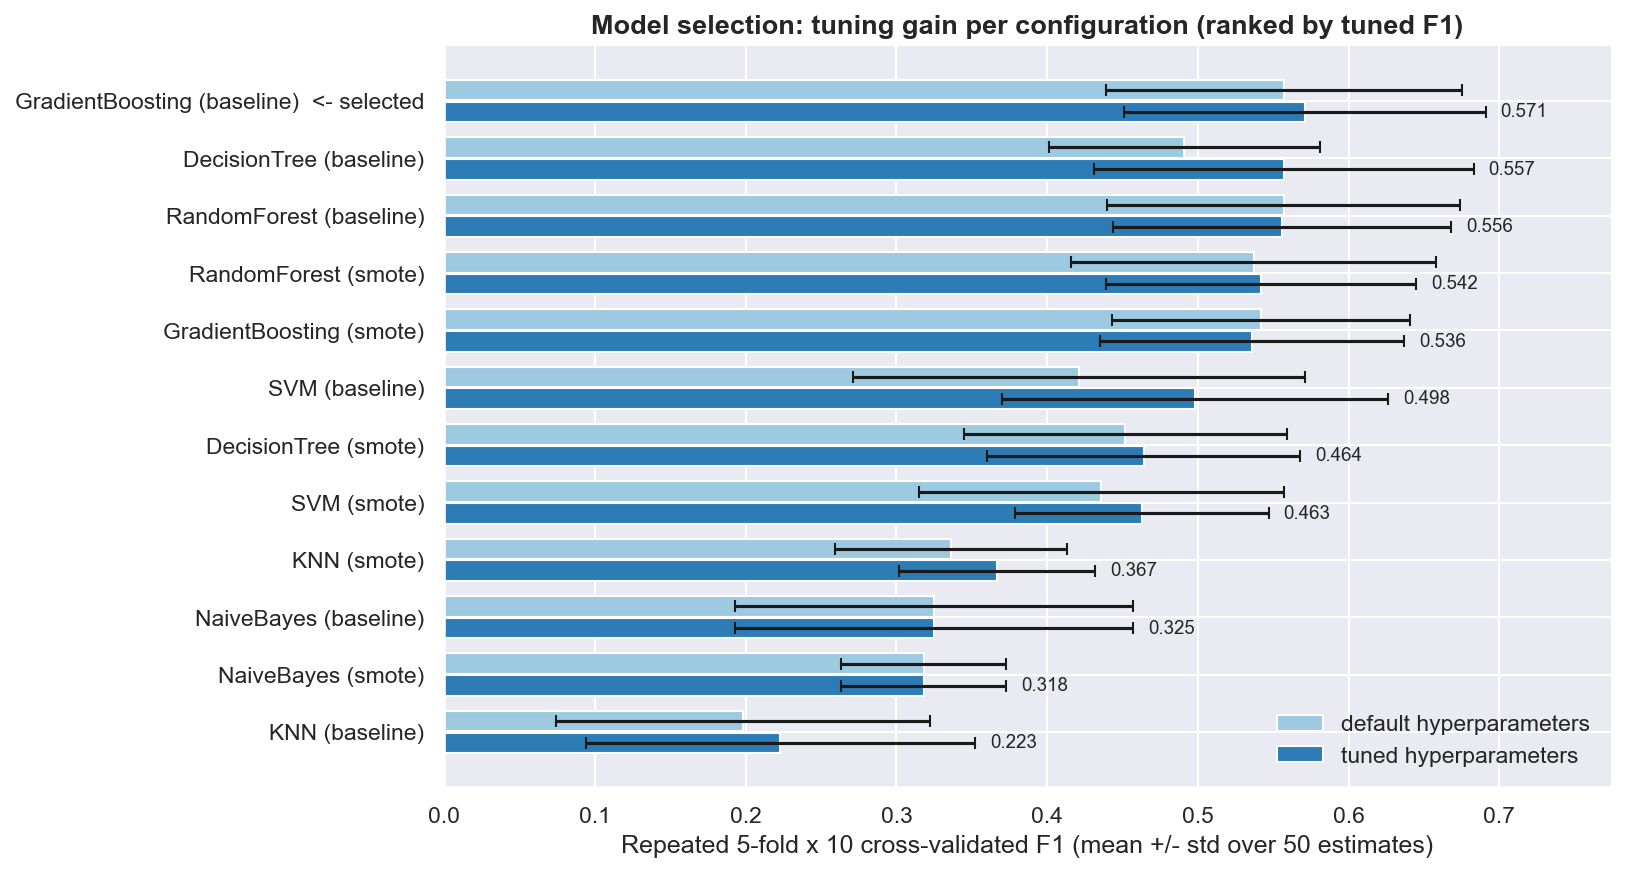
\includegraphics[width=0.9\textwidth]{figures/05_cv_selection.png}
    \caption{Repeated-CV model comparison used for selection}
    \label{fig:cv_selection}
\end{figure}

\section{Threshold-Free Evaluation}
Average precision is the more informative ranking metric here because defaults are rare. The precision--recall curves separate the models less cleanly than the ROC curves, which is expected at an 11\% base rate. Figure~\ref{fig:roc} and Figure~\ref{fig:pr} show the two views, and Figure~\ref{fig:confusion} shows the confusion matrices at the operating points.

\begin{figure}[H]
    \centering
    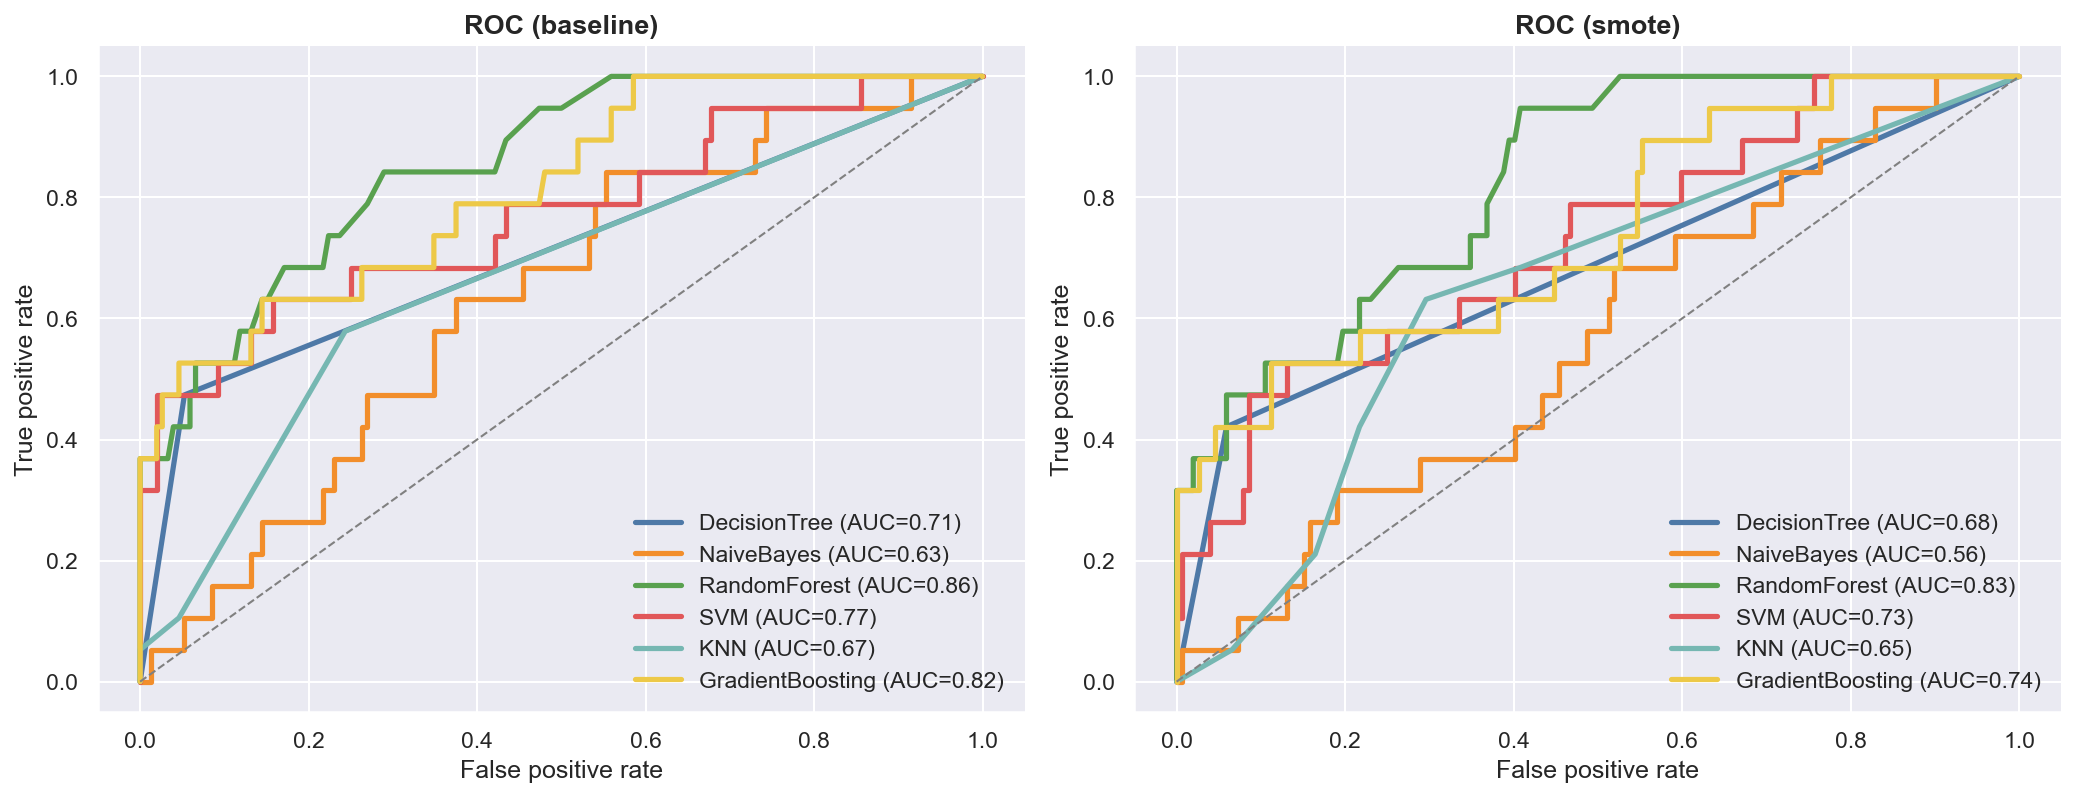
\includegraphics[width=0.85\textwidth]{figures/06_roc_curves.png}
    \caption{ROC curves for the compared classifiers}
    \label{fig:roc}
\end{figure}

\begin{figure}[H]
    \centering
    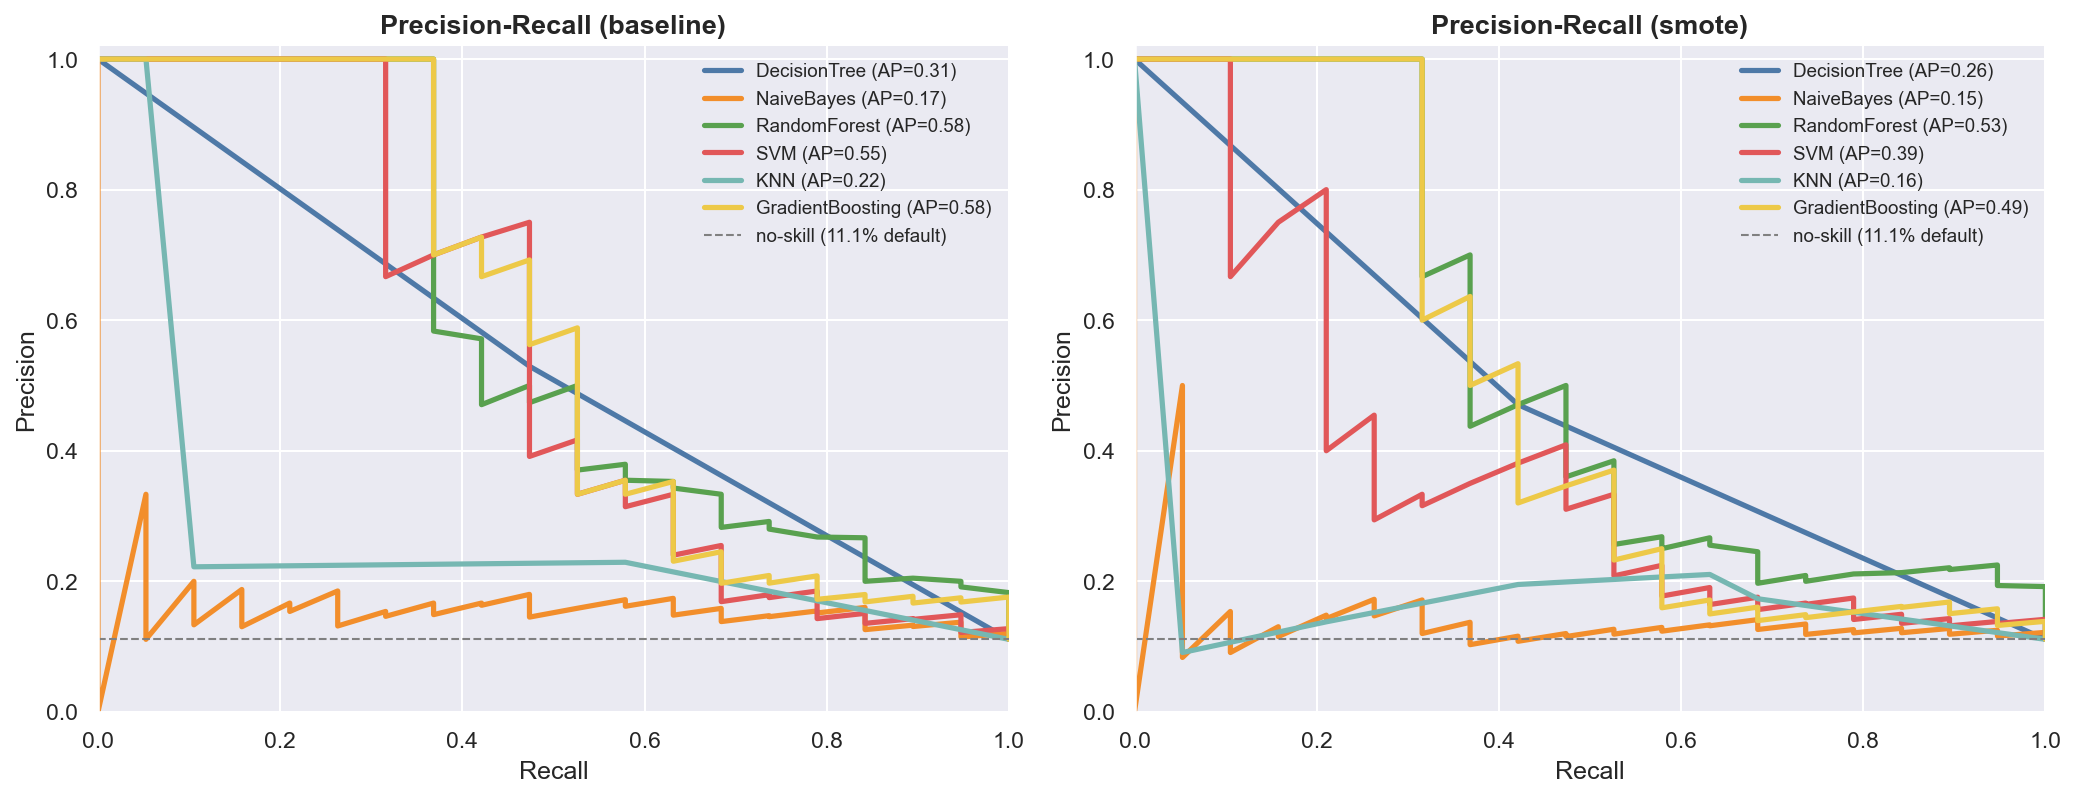
\includegraphics[width=0.85\textwidth]{figures/07_pr_curves.png}
    \caption{Precision--recall curves for the compared classifiers}
    \label{fig:pr}
\end{figure}

\begin{figure}[H]
    \centering
    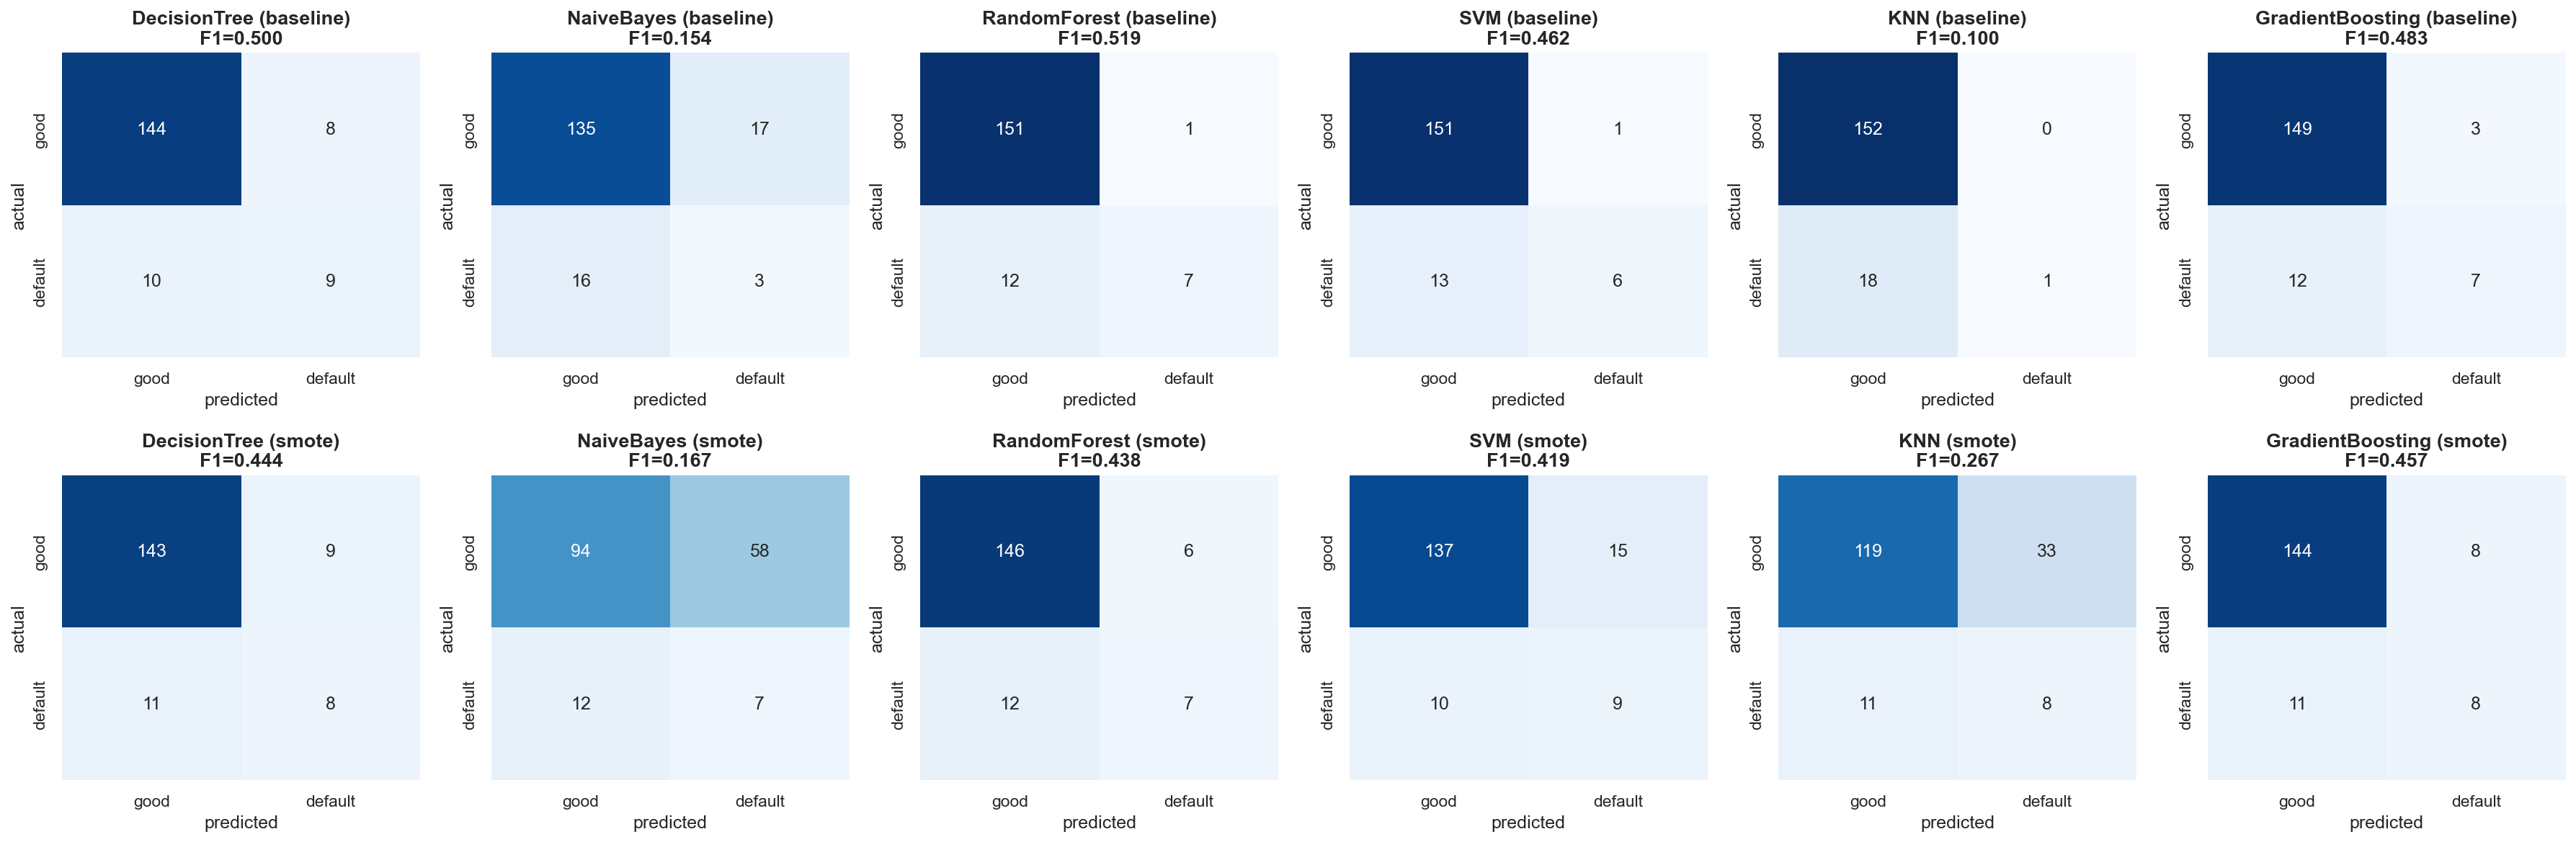
\includegraphics[width=0.88\textwidth]{figures/08_confusion_matrices.png}
    \caption{Confusion matrices at the reported operating points}
    \label{fig:confusion}
\end{figure}

\section{What the Comparison Shows}
\begin{itemize}
    \item SMOTE lowers F1 for five of the six models. It helps KNN, but KNN remains the weakest model.
    \item Hyperparameter tuning materially helps SVM ($+0.077$ F1) and Decision Tree ($+0.066$ F1).
    \item The ensemble models are relatively stable under tuning.
    \item With only 76 defaults, differences below roughly $0.05$ F1 are inside the observed fold-to-fold spread.
\end{itemize}

\begin{figure}[H]
    \centering
    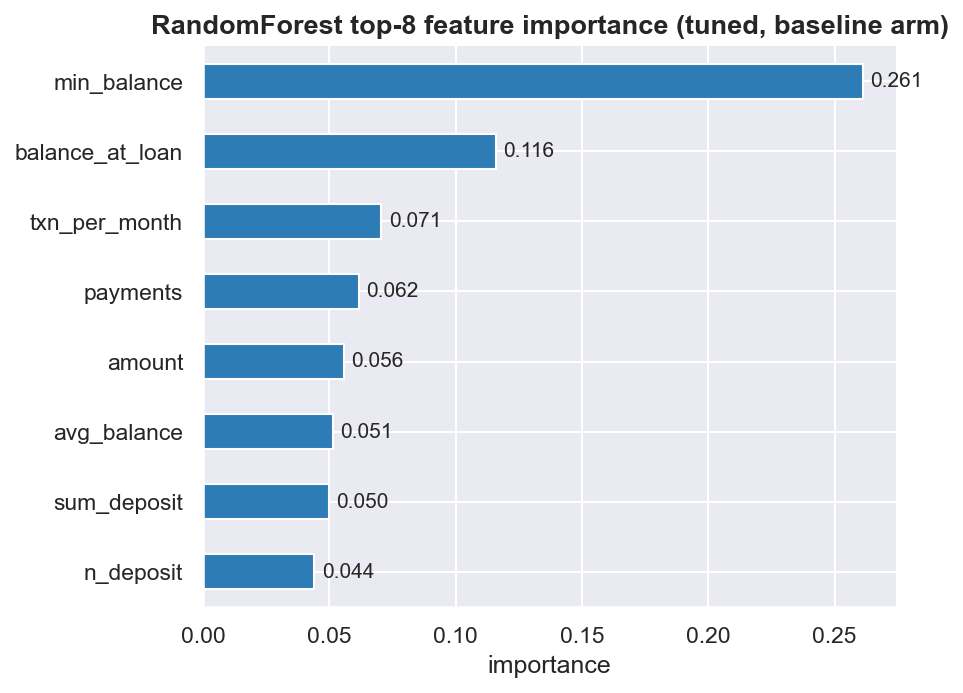
\includegraphics[width=0.85\textwidth]{figures/09_feature_importance.png}
    \caption{Random Forest feature importance}
    \label{fig:importance}
\end{figure}

Random Forest importance agrees with the correlations in Chapter~6: \texttt{min\_balance} leads, followed by \texttt{balance\_at\_loan}, transaction frequency, payments, and amount. Age and gender are close to zero.

\section{Performance Metrics}
The reported classification metrics are defined as follows, with $TP$, $FP$, and $FN$ taken from the confusion matrix:

\begin{itemize}
    \item \textbf{Accuracy:} $(TP + TN) / (TP + TN + FP + FN)$. Limited use here because of class imbalance.
    \item \textbf{Precision:} $TP / (TP + FP)$, the share of flagged loans that actually default.
    \item \textbf{Recall:} $TP / (TP + FN)$, the share of defaults caught.
    \item \textbf{F1:} the harmonic mean of precision and recall; the selection metric.
    \item \textbf{Average precision:} area under the precision--recall curve, more informative than ROC AUC at low base rates.
    \item \textbf{ROC AUC:} probability that a random default scores above a random non-default.
\end{itemize}

All classification metrics come from out-of-fold scores and the held-out split. Clustering metrics, which are internal and do not use the default label, are reported separately in Chapter~9.

\section{Selected Model Implementation}
The tuned Gradient Boosting pipeline is saved with preprocessing included, so a new application is transformed with exactly the same steps used in training. Two challengers were also trained and saved: an MLP neural network and a classification-rule learner (CBA).

\begin{table}[H]
    \centering
    \small
    \begin{tabular}{|l|c|c|c|c|}
        \hline
        \textbf{Model} & \textbf{Precision} & \textbf{Recall} & \textbf{F1} & \textbf{ROC AUC} \\
        \hline
        MLP & 0.694 & 0.329 & 0.446 & 0.750 \\
        CBA rules & $\mathbf{1.000}$ & 0.355 & 0.524 & 0.678 \\
        \hline
    \end{tabular}
    \caption{Additional models}
    \label{tab:additional_models}
\end{table}

The CBA rules are precise but catch only about one third of defaults, and all of them key off a negative minimum balance. That matches both the rule mining and the feature importance. The Simulator page of the dashboard loads the saved Gradient Boosting pipeline, scores one application, places it against the portfolio score distribution, and reports one-at-a-time stress drivers. No model is retrained when the dashboard starts.
